The exploratory pilot showed perfect known-count recovery at $\sigma=0.05$
without added noise. At $q=2$, mean raw K-means ARI was 0.237 for uniform noise
and 0.545 for Gaussian noise; the paired difference was 0.308 (95\% interval
0.181--0.435). After standardization, the corresponding means were 0.970 and
0.999, yet silhouette selected the generating count in 0/20 uniform and 19/20
Gaussian cases. These exploratory observations motivated the independently
seeded validation specified above. Its results and robustness checks will be
inserted from the archived run records after completion and verification.

\begin{figure}[htbp]
\centering
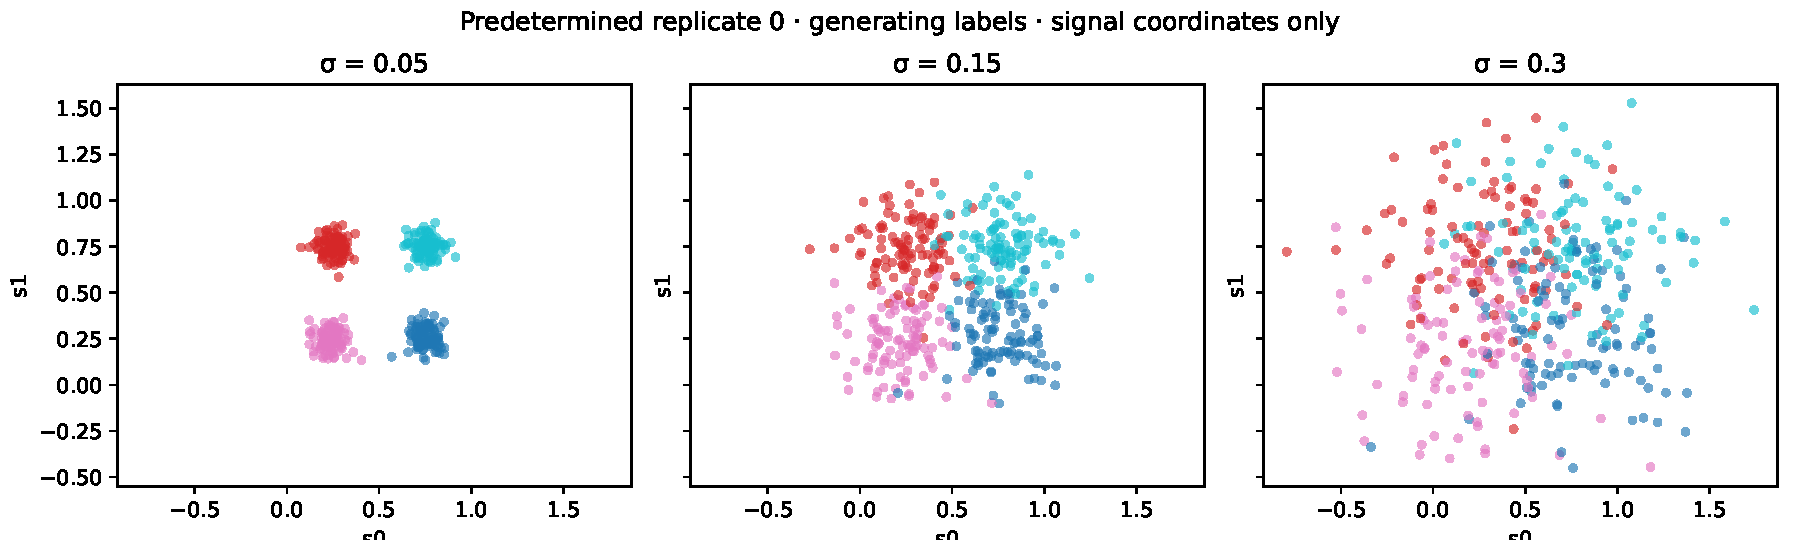
\includegraphics[width=\textwidth]{gallery.pdf}
\caption{Predefined pilot gallery, replicate zero. Each panel shows the first
two signal coordinates, colored by generating label. Adding irrelevant columns
preserves these points; their unchanged appearance is the intended paired
control, not a projection of a changed clustering solution. The exported CSVs
contain the additional coordinates.}
\label{fig:gallery}
\end{figure}
